\chapter{进程}

    \emph{进程是任何躲到程序涉及的操作系统中的基本概念}

\section{进程、轻量级进程和线程}

    OS教科书的常规定义:\emph{进程是程序执行时的一个实例。}每一个进程都只有一个父亲。

    从内核的观点来看:\emph{进程的目的就是担当分配系统资源(CPU time、memory)的实体。}

    对于一个进程的创建,其原理是接受父进程地址空间的一个(逻辑)拷贝。\emph{尽管父子进程可以共享含有程序代码(正文)的页,但是拥有各自独立的数据拷贝,因此子进程对内存单元的修改对父进程是不可见的(反之亦然)}

    对于现代Unix系统来说,需要支持多线程应用————\emph{拥有很多相对独立执行流的用户程序共享应用的大部分数据结构。}这样的系统中,进程由多个线程组成,每个线程都代表进程的一个执行流。

    目前而言,大多数多线程应用都是基于pthread(POSIX thread)库的标准库函数集编写的

    Linux使用轻量级进程(lightweight process)对多线程进行更好的支持。\emph{对于轻量级进程而言,可以共享资源,只要其中一个修改共享资源,另一个就会立即查看并同步。}

\subsection{进程描述符}

    进程描述符(process descriptor,由task\_struct类修饰),其字段包含了与进程相关的所有信息。

\begin{figure}[!htbp]
    \centering
    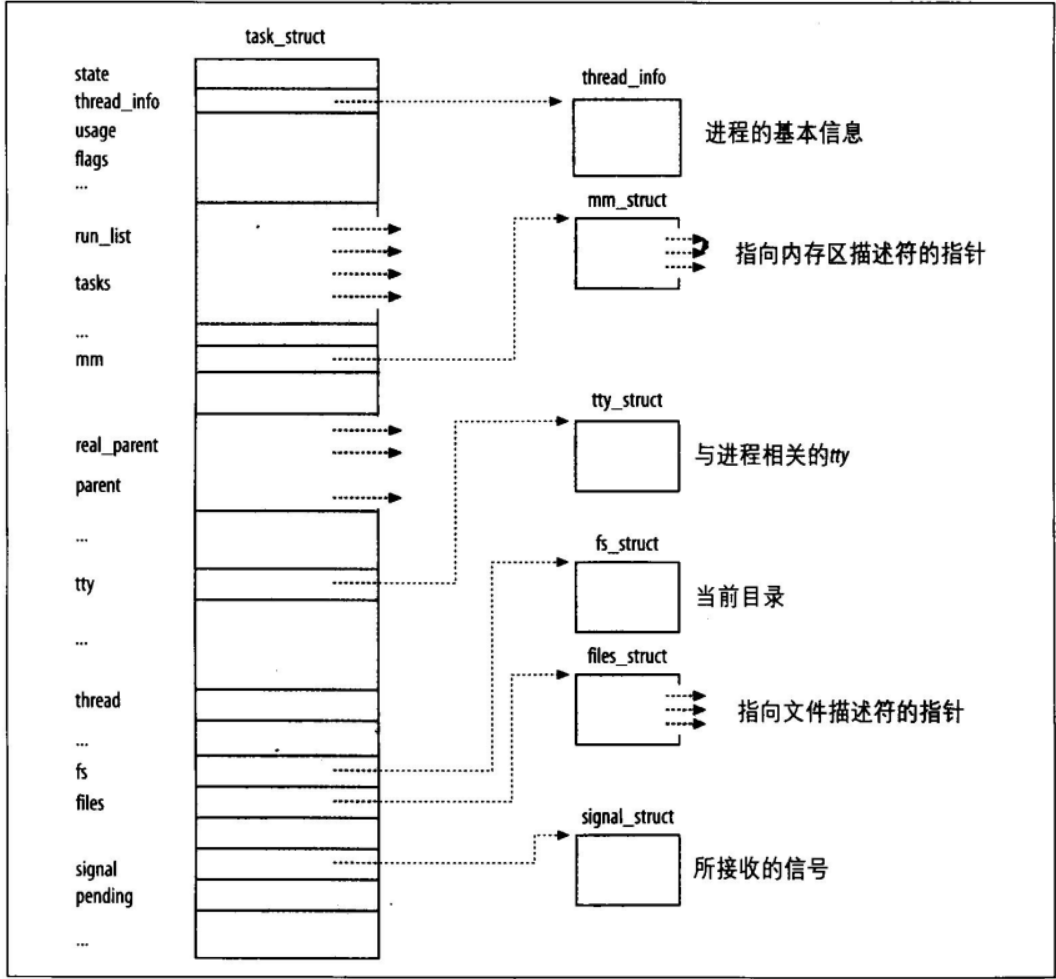
\includegraphics[width=0.8\textwidth]{image/chapter03/Linux进程描述符.png}
    \caption{Linux进程描述符}
\end{figure}

    图3-1右边的六个数据结构涉及进程拥有的所有特殊资源,目前我们只讨论两种:进程的状态以及进程的父子关系

\subsection{进程状态}

    进程描述符中的state字段描述了当前进程所处的状态。其由一组标志组成,其中每一个标志描述了一种可能的进程状态。

    值得注意的是:\emph{状态之间是互斥的,严格意义上只允许存在一种状态。}

\begin{lstlisting}[language=C++, caption={进程状态一览}]
#define TASK_RUNNING		    0
#define TASK_INTERRUPTIBLE	    1
#define TASK_UNINTERRUPTIBLE	2
#define TASK_STOPPED		    4
#define TASK_TRACED		        8
#define EXIT_ZOMBIE		        16
#define EXIT_DEAD		        32
\end{lstlisting}

\begin{itemize}
    \item TASK\_RUNNING
    \subitem 进程要么已经执行,要么准备执行
    \item TASK\_INTERRUPTIBLE
    \subitem 进程被挂起,知道某个条件为真。产生硬件中断,释放进程正在等待的系统资源或传递一个信号都是可以唤醒进程的条件(也就是恢复到TASK\_RUNNING)
    \item TASK\_UNINTERRUPTIBLE
    \subitem 与上一个状态类似,但传递信号无法唤醒。\emph{一般用于特殊情况下,进程必须等待,直到一个不能被中断的实践发生}
    \item TASK\_STOPPED
    \subitem 进程的执行被暂停,当接收到SIGSTOP、SIGTSTP、SIGTTIN和SIGTTOU信号后,进入暂停
    \item TASK\_TRACED
    \subitem 进程的执行由debugger程序暂停。当一个进程被另一个进程监控时,任何信号都可以把这个进程置于TASK\_TRACED状态
    \item EXIT\_ZOMBIE
    \subitem 进程的执行被终止,但是父进程未发布wait()类系统调用来返回有关死亡进程的信息
    \item EXIT\_DEAD
    \subitem 最终状态,由于父进程刚发布wait()类系统调用,因而进程被系统删除,但防止其他线程也执行wait()类系统调用,为了防止冲突,因而将僵死状态设置为僵死撤销(将亡)状态
\end{itemize}

    一般的,进程状态可以由以下简单的赋值语句设置,也可以由宏设置:

\begin{lstlisting}[language=C++]
p->state = TASK_RUNNING;

#define __set_task_state(tsk, state_value)		\
	do { (tsk)->state = (state_value); } while (0)
#define set_task_state(tsk, state_value)		\
	set_mb((tsk)->state, (state_value))

#define __set_current_state(state_value)			\
	do { current->state = (state_value); } while (0)
#define set_current_state(state_value)		\
	set_mb(current->state, (state_value))
\end{lstlisting}

\subsection{标识一个进程}

    进程和进程描述符之间有非常严格的一一对应关系,这使得进程描述符标识进程称为一种方便的方式。

    另一方面,类Unix操作系统允许用户使用进程标识符process ID(PID)来标识进程,PID存放在进程描述符的pid字段中。

    PID被顺序编号,新创建的进程通常是前一个PID加1。PID的值通常有一个上线,缺省情况下,最大PID号是32767(PID\_MAX\_DEFAULT - 1)

    由于循环使用PID,因此需要通过与个pidmap\_array位图来标识当前已分配的PID和闲置的PID。

    Linux希望同一个线程组内有同一个PID,因此,\emph{一个线程组中的所有线程使用和该线程组的领头线程的PID,被存放在进程描述符中的tgid字段。}系统调用getpid()实际上是返回的tgid的值,而非PID。

\subsection{进程描述符处理}

    进程是动态实体,因此内核必须能够同时处理多进程,并把进程描述符存放在动态内存中,而非在永久分配给内核的内存区。

    对于每个进程来说,Linux把内核态的进程堆栈和进程描述符中的thread\_info(线程描述符)紧凑的存放在一个单独的存储区域内。

\begin{figure}[!htbp]
    \centering
    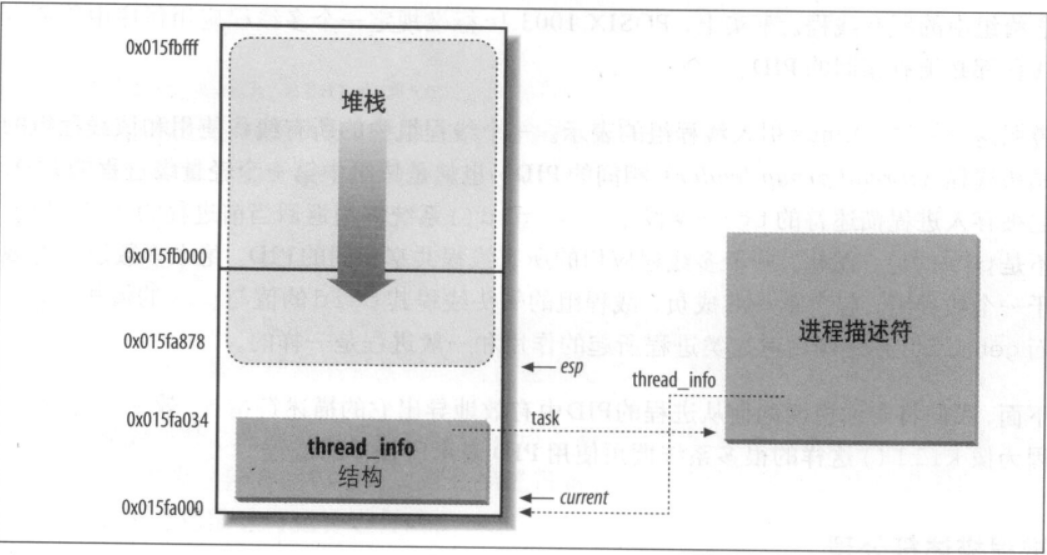
\includegraphics[width=0.8\textwidth]{image/chapter03/thread_info与进程内核栈.png}
    \caption{thread\_info结构和进程内核栈存放在两个连续的页框中}
\end{figure}

    线程描述符驻留于该内存区的开始,栈从末端向下开始增长。

    esp寄存器是CPU的栈指针(x86架构),用来存放栈顶单元的地址。栈起始于末端,并朝该内存区开始的地方开始增长。\emph{从用户态切换到内核态后,进程的内核总是空的}

    在内核中,使用union对该结构进行描述:

\begin{lstlisting}[language=C++]
#define THREAD_SIZE     (4096)
#else
#define THREAD_SIZE		(8192)
#endif

union thread_union {
    struct thread_info thread_info;
    unsigned long stack[THREAD_SIZE/sizeof(long)];
};
\end{lstlisting}

\subsection{标识当前进程}

    从效率上看:\emph{thread\_info结构体与内核态堆栈之间的紧密结合提供的主要好处为:内核可以轻易从esp的值获取CPU正在运行进程的thread\_info的地址}

    事实上,如果thread\_union结构长度是8K($2^{13}$),则内核屏蔽掉esp的低13位有效位就能够获取thread\_info的基地址。这项工作由以下函数实现:

\begin{lstlisting}[language=C++]
/* how to get the thread information struct from C */
static inline struct thread_info *current_thread_info(void)
{
    struct thread_info *ti;
    __asm__("andl %%esp,%0; ":"=r" (ti) : "0" (~(THREAD_SIZE - 1)));
    return ti;
}
\end{lstlisting}

    也就是说,通过该函数内联汇编:

\begin{lstlisting}[language=C++]
movl $0xffffe000, %ecx
andl %esp, %ecx
movl %ecx, p
\end{lstlisting}

    这样执行后,p就包含了CPU当前运行进程的thread\_info结构的指针。

    但是,进程中最常用的是进程描述符的地址而非thread\_info的地址,因此,内核需要调用current宏,其等价于

\begin{lstlisting}[language=C++]
current_thread_info()->task;

movl $0xffffe000, %ecx
andl %esp, %ecx
movl (%ecx), p
\end{lstlisting}

    查看源码可以知道,task在thread\_info上的偏移量是0,因此上述三条指令就能够将进程描述符指针赋值到p上。

    